% =============================================================================
% SEÇÃO 3.1: AUDITORIA DE SIGNIFICÂNCIA ESTATÍSTICA (PESSOA 1 — LUCAS)
% Formato Condensado: 2 Páginas ACM sigconf
% =============================================================================

\subsection{Statistical Audit Framework (Miller, 2024)}
\label{sec:stat_methodology}

To audit claimed downstream parity~\cite{foroutan2026parity}, we implement Miller's super-population framework~\cite{miller2024adding}. Because model $A$ (PA-BPE) and baseline $B$ (Classical BPE) are evaluated on identical prompts, analyzing paired differences $d_i = s_{A,i} - s_{B,i}$ isolates model variance (Miller Eq.~7):
\begin{equation}
\mathrm{SE}_{A-B,\mathrm{paired}} = \sqrt{\mathrm{SE}_A^2 + \mathrm{SE}_B^2 - 2\rho\,\mathrm{SE}_A\mathrm{SE}_B}.
\label{eq:paired_se}
\end{equation}
Crucially, multilingual benchmarks translate identical questions $c \in \{1,\dots,C\}$ across languages. Treating them as independent violates the Central Limit Theorem. We apply the paired, cluster-adjusted standard error (Miller Eq.~8):
\begin{equation}
\mathrm{SE}_{A-B,\mathrm{clustered}} = \frac{1}{n}\left(\sum_{c=1}^{C}\sum_{i \in c}\sum_{j \in c}(d_{i,c} - \bar{d})(d_{j,c} - \bar{d})\right)^{\!1/2}\!\!,
\label{eq:clustered_se}
\end{equation}
yielding cluster-robust 95\% confidence intervals $\bar{d} \pm 1.96\,\mathrm{SE}_{\mathrm{clustered}}$.

\begin{figure}[t]
    \centering
    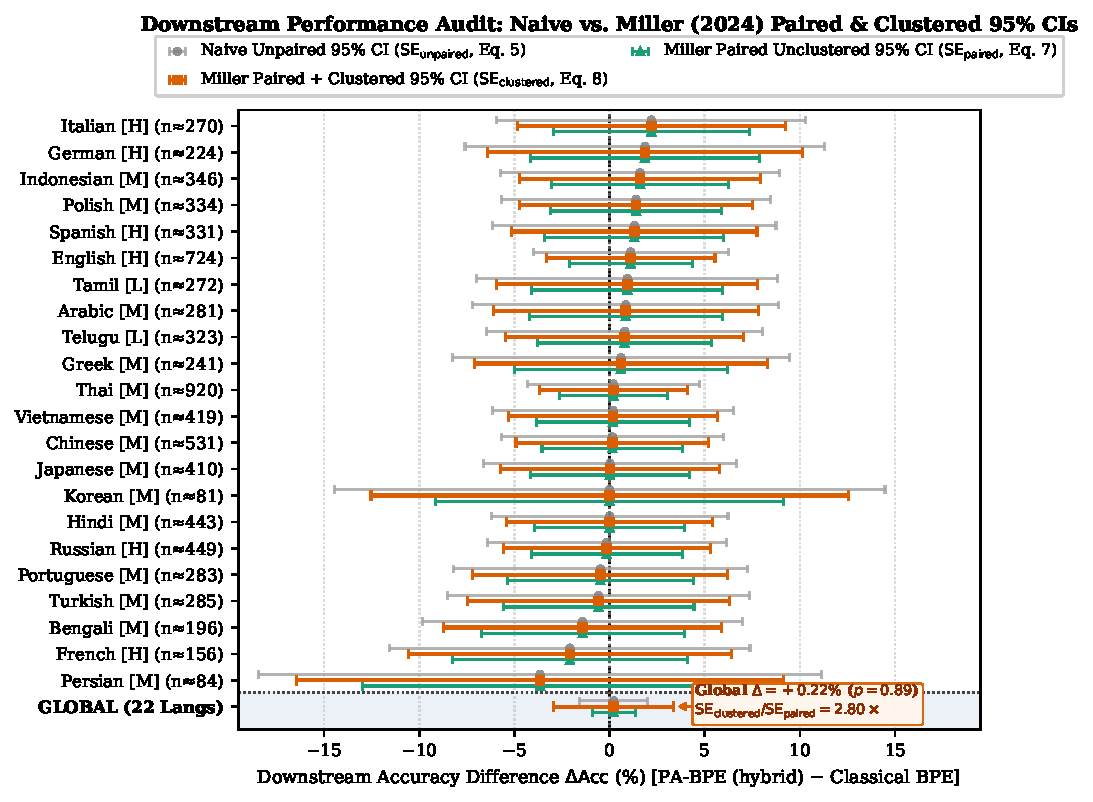
\includegraphics[width=0.98\columnwidth]{figures/fig1_forest_plot.pdf}
    \vspace{-1.2em}
    \caption{Downstream $\Delta\mathrm{Acc}$ (\textbf{PA-BPE hybrid $-$ Classical BPE}) across 22 languages. Clustering inflates global uncertainty by $\mathbf{2.80\times}$; all 22 languages cross zero at 95\% CI.}
    \label{fig:forest_plot}
    \vspace{-0.6em}
\end{figure}

\subsection{Downstream Significance Audit Results}
\label{sec:results_significance}

Figure~\ref{fig:forest_plot} presents our audit of Table~2 from~\cite{foroutan2026parity}. Inverting Bernoulli SEs ($\sqrt{\bar{s}(1-\bar{s})/n}$) uncovers an $11\times$ effective sample disparity: Korean ($n_{\mathrm{eff}} \approx 81$) and Persian ($n_{\mathrm{eff}} \approx 84$) span 1 benchmark, while English ($n_{\mathrm{eff}} \approx 724$) and Thai ($n_{\mathrm{eff}} \approx 920$) span 10--11.

Accounting for pairing ($\rho = 0.60$) reduces SEs by $36.8\%$, but cluster adjustment reverses this gain. In the global 22-language aggregate ($\Delta\mathrm{Acc} = +0.22\%$), unclustered paired SE is $\pm 0.57\%$ ($z = 0.38$), but clustering by parallel question inflates uncertainty by $\mathbf{2.80\times}$ to $\mathrm{SE}_{\mathrm{clustered}} = \pm 1.60\%$ ($z = 0.14, p = 0.89$). Across a sensitivity sweep ($\rho \in [0.0, 0.8]$), \textbf{0 out of 22 languages} exhibit statistically significant differences ($p > 0.05$). Nominal gains (Italian $+2.19\%$, German $+1.86\%$) and declines (Persian $-3.65\%$) represent random evaluation noise.
